% Co udělal někdo jinej
\chapter{Rešerše ($\sum$ = 16 stran)} \label{chap:Rešerše}
\section{Frekvenční měniče a jejich role v řízení dopravníků ($\sum$ = 3 strany)}\label{sec:FrekvencniMeniceAJejichRole}
\purpose{Vysvětlit s jakým systémem už pracuji}

Dopravníky společnosti Honeywell obsahují asynchronní motory. Na těchto motorech lze nastavovat rychlost pomocí frekvenčních měničů a tyhle frekvenční měniče lze řídit pomocí PLC. Spolu s těmito motory mají dopravníky hodně převodů a další mechanismy, které umožňují pohyb balíků na dopravnících. Dopravníky jsou buďto pásové anebo rollerové (válcové) což ovlivňuje moment na motoru a další. Tohle tady ale víc nemám v plánu vysvětlovat.

Frekvenční měniče jsou v běžném provozu řízené komunikační linkou, která komunikuje přes Profinet (industriální komunikační sběrnice používaná pro průmyslovou automatizace). Profinet se programuje přes program Siemens Tiaportal, což je prostředí vyvinuté od Siemens právě pro řízení různých frekvenčních měničů pomocí Siemens PLC. V tomto programu lze modelovat a řídit celou dopravníkovou linku.

Tohle zařízení se ale nenavrhuje pro běžný provoz dopravníků, protože ten je řízený těmi PLC. Tahle deska se navrhuje pro zjednodušení kontroly dopravníků během testování funkčnosti po tom co jsou dopravníky nainstalovány ve skladech zákazníků. V rámci zkoušek není potřeba aby spolu frekvenční měniče komunikovali přes Siemens PLC, ale je víc důležitější aby bylo možné kterýkoliv frekvenční měnič spustit a aby na to existoval návod, který jsou schopni plnit i osoby co nemají vzdělání v rámci PLC, jako třeba mechaničtí inženýři.

V rámci rešerše se přišlo na to, že ovládací panel frekvenčního měniče lze resetovat do různých defaultních nastavení. Jedno z těchto nastavení je "Default setting no. 9", které umožňuje ovládat frekvenční měnič přes vstupy, které jsou na ovládacím panelu. Tenhle reset ovládacího panelu je navíc možný pomocí Siemens Intelligent Operator Panel 2 (IOP-2), což je zařízení které existuje právě aby bez inicializace Profinetu umožnilo změny nastavení ovládacího panelu frekvenčního měniče.

\source{Tady mám jako zdroje siemens web a datasheety}

\begin{itemize}
    \item Frekvenční měnič, který ovládám: Sinamics G120D
    \item Tenhle frekvenční měnič má ovládací panel: CU240D-2 \cite{SiemensG120DGettingStarted}
\end{itemize}
\begin{figure}[H]
    \centering
    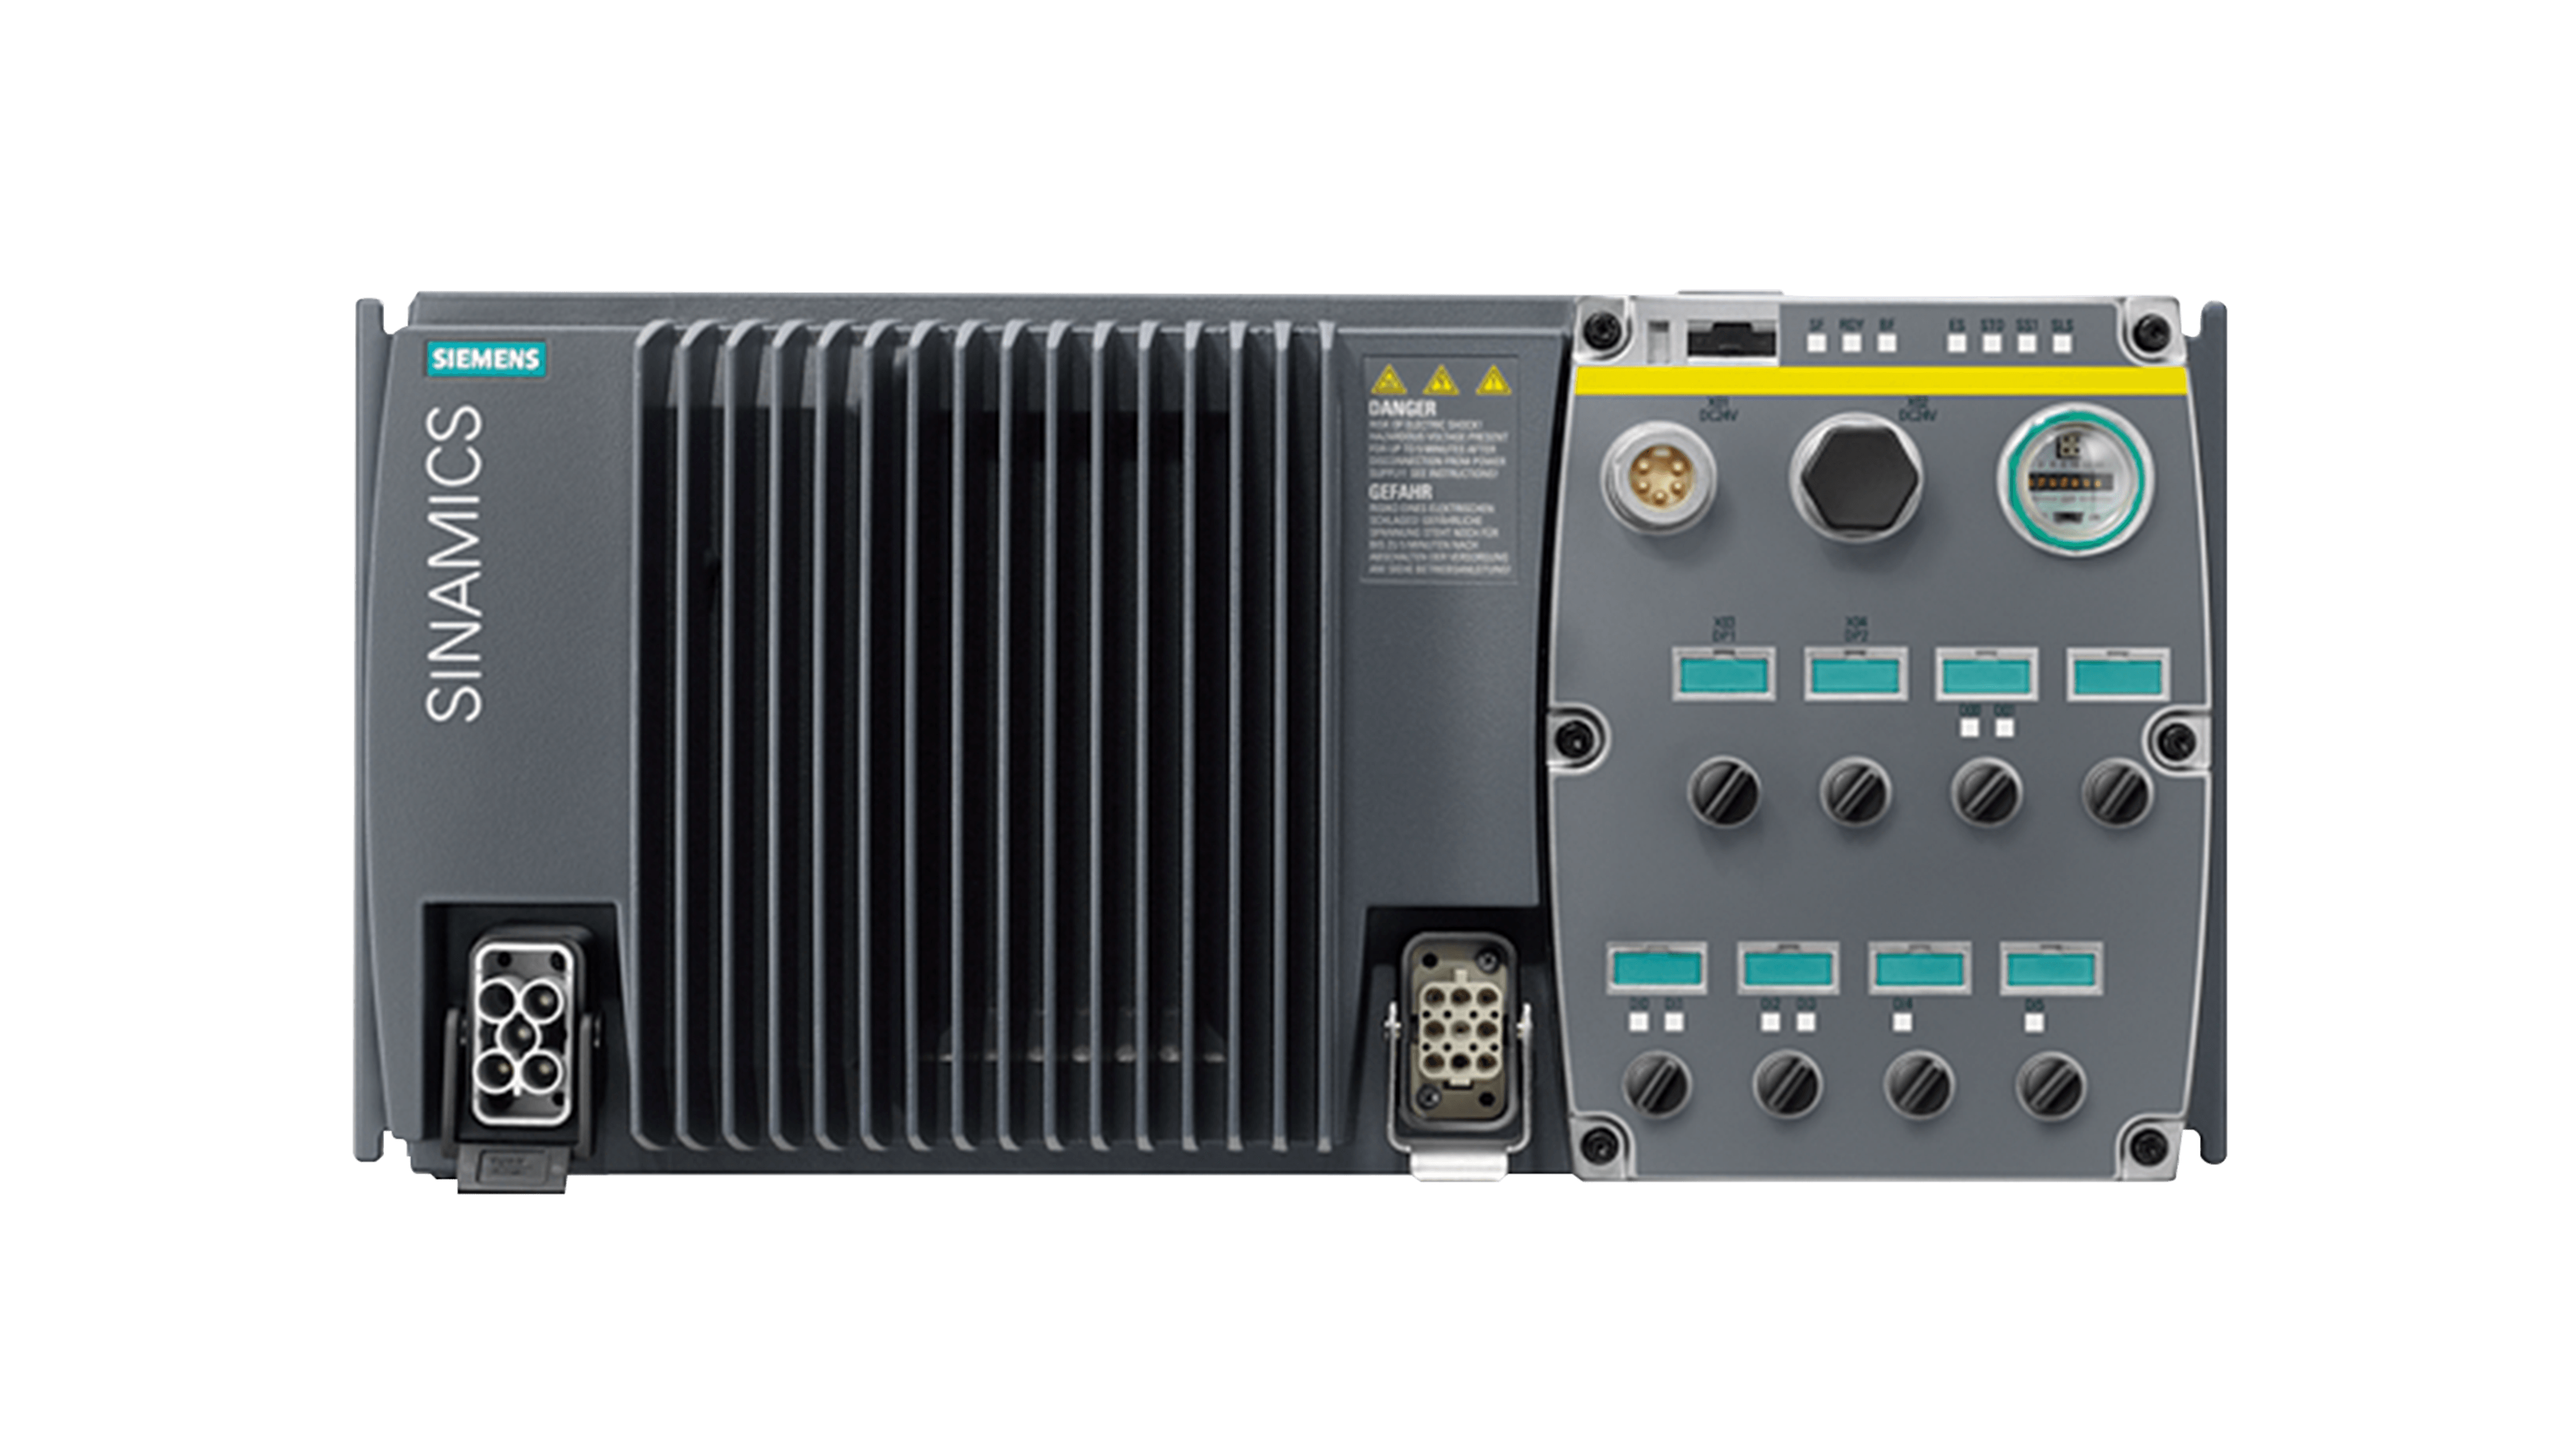
\includegraphics[width=0.8\linewidth]{images/Sinamics_G120D.png}
    \caption{Frekvenční měnič Sinamics G120D \cite{SinamicsG120D}}
    \label{fig:sinamics_G120D}
\end{figure}

\subsection{Jak frekvenční měniče fungují}\label{sec:JakFungujiFrekvencniMenice}
\purpose{Vysvětlit jak vlastně ten frekvenční měnič funguje a proč ho používáme v dopravnících}

V dopravnících frekvenční měnič nemusí být a můžeme napájet rovnou motorem, ale potom by nebylo možné mít tak robustní řídící systém, protože by byly motory v dopravnících mnohem hůř ovladatelné.

\subsection{Detailnější popis Sinamics G120D}
\purpose{Popsat hlavní parametry frekvenčního měniče - rozsah napájecího napětí, maximální proud, podporovaný komunikační protokoly (Profinet) - nějaký basic info o Sinamics G120D. Tady přidat i to že Sinamics G120D pracuje s asynchronními motory - jaké jsou od Siemens třeba nejčastější?}


\subsection{Nastavení ovládacího panelu (1.5 strany)}\label{sec:NastaveniOvladacihoPanelu}
\purpose{Vysvětlit jak se dají dopravníky nastavit aby fungovaly s mým systémem}

Ovládací panel se může nastavit pomocí Siemens Tiaportal anebo pomocí Sinamics IOP‑2 Intelligent Operator Panel, kterej se připojí přes optický kabel. Zde je postup nastavení:\cite{SiemensG120DGettingStarted}
\begin{itemize}
    \item IOP-2 se připojí na kontrolní panel pomocí optického kabelu
    \item V IOP-2 se zresetuje nastavení VFD
    \item Vybere se nastavení Default setting 9: "Standard I/O with MOP" 
    \item Zbytek nastavení je možné nechat na defaultních nastaveních
    \item Nyní je možné IOP-2 odpojit od frekvenčního měniče
\end{itemize}

Díky tomuto je nyní ovládací panel frekvenčního měniče nastaven tak, aby bylo možné ho ovládat těmito digitálními signály na jeho vstupy:
\begin{itemize}
    \item Pokud je DI0 HIGH, frekvenční měnič je zapnutý.
    \item Pokud je DI1 HIGH, bude růst rychlost dopravníku.
    \item Pokud je DI2 HIGH, bude rychlost dopravníku zpomalovat.
\end{itemize}

\subsubsection{Možnosti dalších default nastavení ovládacího panelu}
\purpose{popsat nastavení default with potentiometer a default MOP with E-STOP}

V rámci návrhu systému je možné použít defaultní nastavení které umožňuje připojení potenciometru k analogovému portu ovládacího panelu. V takovém případě by se rychlost mohla nastavovat přímo potenciometrem. Schránka na desku by tak neměla dvě tlačítka na zrychlení a zpomalení, ale jen jedno, ale zároveň by to zhoršovalo dálkové ovládání, protože to se dělá jednodušeji pokud posílám pouze digitální výstupy.

také je možné použít ještě možnost defaultního nastavení s E-STOP. To by nastavilo nějaký digitální vstupy jako E-STOP vstupy, které by musely být napojený na E-STOP který má sepnuté kontakty pokud není zmáčknutý. Tohle byla původní možnost návrhu, ale tenhle E-STOP by zabíral hodně místa na fyzické schránce systému a tento bezpečnostní prvek je stejně rozmístěný všude kolem dopravníků a už i v commisioning fázi je funkční a schopný dopravník okamžitě zastavit.

S tímto je tedy nejjednodušší použít setting který jsem si zvolil.

\subsection{Bezpečnostní aspekty práce s ovládacím panelem}
\purpose{Zmínit že když pracuji s takovýmto výkonovým zařízením, musím si dát pozor na bezpečnost. Vysoký napětí který vystupuje z frekvenčního měniče se dá vypnout přepínačem který je umístěný nad ovládacím panelem. Potom už člověk pracuje jen s 24V které jsou na všech portech ovládacího panelu a kvůli tomu všechny porty zakrývají šroubovací gumové kryty, které je potřeba oddělat předtím než se můžou připoji kabely ze systému co navrhuji.}

\section{Open source vývojové desky ($\Sigma$ = 6 stran)}
\purpose{Zde bude úvod do open source vývojových desek.} 

Nejznámnější návrhář těchto desek je Arduino, já ale používám WEMOS.

Jejich velká výhoda jsou integrované USB porty a extra rozhraní a specifikace, díky čemuž je můžu používat bez toho, abych si musel integrovat vlastní obvod s mikrokontrollerem do desky. Navíc pokud do desky pouze napájím kolíkovou lištu a ne rovnou celou vývojovou desku, můžu vývojovou desku v případě poruchy rychle vyměnit.

Proč jsem se rozhodl pro open source vývojové desky? Dostupnost, flexibilita a že se přesně můžu podívat na to jak ta deska funguje - což se hodí při návrhu desky plošných spojů, protože přesně vím jak ta deska funguje jelikož se můžu podívat na schematic. Navíc jelikož jsou tyhle systémy open source, mám možnost využívat již existujících balíčků pro rozšíření funkčností mikrokontrollerů co jsou na desce uloženy - knihovny jako třeba Ticker která je popsána v sekci \ref{sec:TickerKnihovna} anebo kód pro jednoduché používání koupeného LCD displeje bez nutnosti programovat jeho ovládání pomocí I2C od základu.

\source{Tady zkusím najít nějaký zdroj z knihovny - nějaká knížka o arduinu}

\subsection{Proč WEMOS vývojové desky (1.5 strany)}
\purpose{Tady bude popsané co jsou WEMOS desky a proč je používám. Taky tady bude důvod proč jsem si vybral WEMOS D1 Mini pro a srovnání s wemos D1 mini a arduino UNO}

WEMOS desky jsou vývojové desky co používají mikrokontrollery ESP32 nebo ESP8266 a mají v sobě integrované i WiFi moduly, což běžné arduino vývojové desky většinou nemají. Jsou také open source stejně jako arduino a tak jsou lehce dostupné, protože mohou firmy vytvářet svoje vlastní klony.

Je možné je programovat pomocí arduino IDE a arduino jazyka (variace na C++). Já je programuji skrz alternativu Arduino IDE jménem Platformio.

můžu ukázat wemos d1 mini základní web script tam kde bude zmíněný \cite{NavodNaESPWebServerDratek}

\source{Tady budou zase online zdroje, protože jsem zase neviděl moc knížek co by nějak vysvětlovali co jsou WEMOS desky}

\begin{figure}[H]
    \centering
    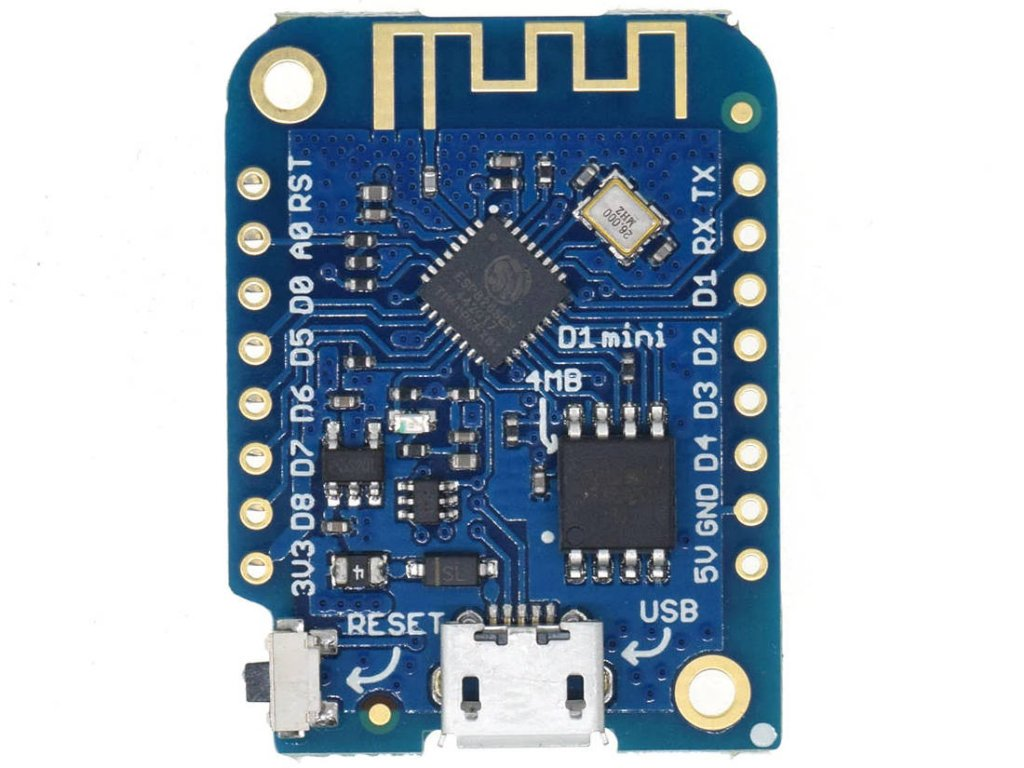
\includegraphics[width=0.5\linewidth]{images/WEMOS_D1_Mini_Pro.jpg}
    \caption{Použitá varianta vývojové desky WEMOS D1 Mini Pro \cite{WEMOSD1MiniPro}}
    \label{fig:WEMOSD1MiniPro}
\end{figure}

\subsection{Technické specifikace WEMOS D1 Mini Pro}
\purpose{Rozvinout co jsou specifikace D1 Mini Pro a co ty jednotlivé věci znamenají - počet GPIO, I2C, PWM, paměť, typ mikrokontrolleru, atd. - nějaký základní basic informace}

\subsubsection{Architektura ESP8266 a srovnání s ESP32}
\purpose{Vysvětlit jak se liší ESP32 a ESP8266 a proč se ESP8266 víc hodí pro tento projekt - ESP32 má wifi i bluetooth a ESP8266 má jen wifi. Zdroj needed.}

\subsection{Arduino jazyk a Platformio (3 strany)}
\purpose{Vysvětlení že existuje arduino jazyk a na čem je založen, zmínění že existuje Arduino IDE a vysvětlení základu jak funguje platformio a jak se liší od Arduino IDE.}

\purpose{Vysvětlení že existují soubory funkcí a hlavičkové soubory.}

\source{Tady možná budu muset mít internetový zdroje, protože jsem nenašel žádnou publikaci co by mluvila o Platformio.}

\begin{figure}[H]
    \centering
    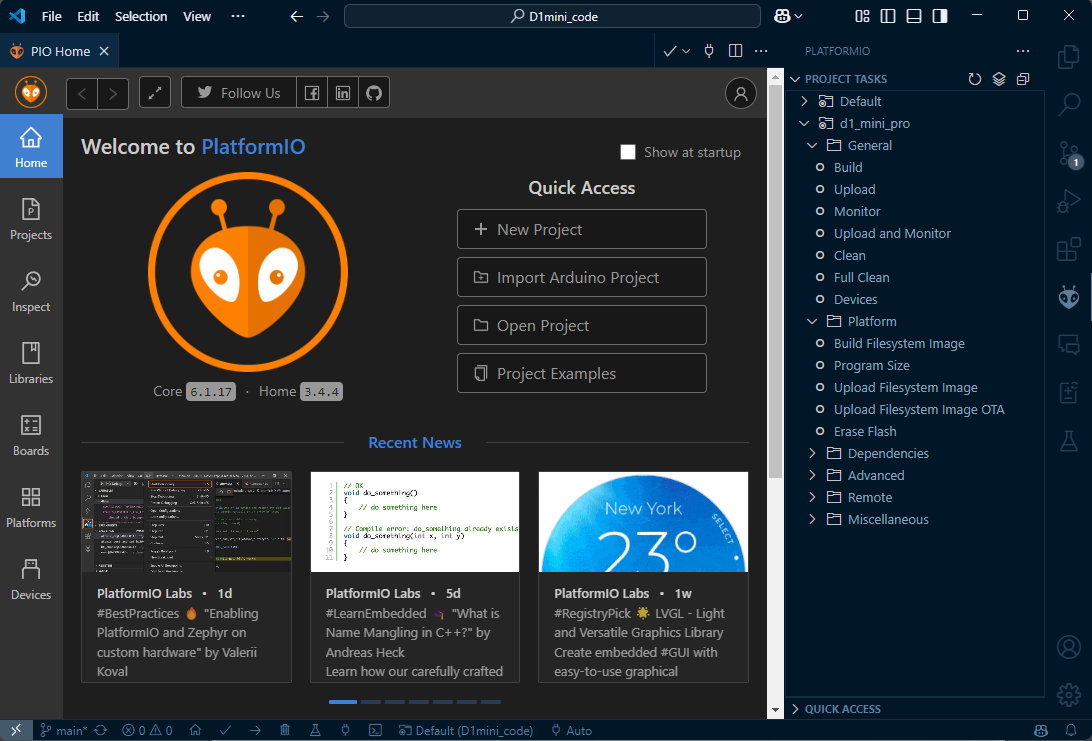
\includegraphics[width=0.9\linewidth]{images/Platformio_Ukazka.png}
    \caption{Ukázka rozhraní vývojového prostředí Platformio}
    \label{fig:PlatformioUkazka}
\end{figure}

\subsubsection{Objekty v arduino C++ jazyce}
\purpose{Tady bych rád vysvětlil jak fungují objekty v arduino C++ jazyce jelikož je využívám uvnitř kapitoly \ref{sec:ConveyorController}. }

U objektů jde obecně jde hlavně o to, že si můžu vytvořit globální instanci objektu a tam si zadefinovat public metody a public proměnné (které můžu zavolat a získat přímo z objektu a používat v main kódu) a private metody a private proměnné (které jsou dostupné jenom uvnitř objektu, takže je můžu získat jen vevnitř jiných metod a proměnných).

\subsubsection{Ticker knihovna}\label{sec:TickerKnihovna}
\purpose{Podobně jako existuje timer u microchip MCU existuje i timer knihovna zvaná Ticker u MCU co se programují v arduino jazyce. Tuhle knihovnu já používám a zmiňuju v sekci \ref{sec:ImplementaceConveyorControllerVeMainCpp} a tak se hodí ji trochu vysvětlit.}

Vývojové desky kompatibilní s platformou Arduino umožňují integraci knihovny Ticker, která poskytuje mechanismus načasování funkcí v definovaných intervalech bez blokování provádění zbytku kódu. Pokud by byla použita funkce \texttt{delay()}, mohlo by to vést ke dvěma problémům. Prvním je různý čas délky vykonávání kódu, které by zesložiťovala spolehlivé nastavení přesných časových intervalů. Druhým problémem je blokující povaha funkce \texttt{delay()}, která by znemožnila časově kritické operace, jako je například reakce na síťové požadavky na serveru nodeMCU běžícím na mikrokontrolrru, což by mohlo zpomalit funkčnost celého systému. \cite{TickerKnihovna}

Je tedy možné se spolehnout na to, že se bude prováděná funkce spouštět přesně ve stanovený čas, což umožňuje aproximaci rychlosti dopravníku která je popsána v kapitole \ref{sec:AproximaceRychlostiDopravniku}.

Pro použití Ticker knihovny je potřebné si knihovnu nejdříve importovat pomocí příkazu \texttt{\#include "Ticker.h"} v záhlaví souboru a následně je možné ji nastavit v \texttt{setup()} funkci hlavního skriptu.

\begin{lstlisting}[language=C++, caption={Použití ticker knihovny uvnitř \texttt{setup()} funkce \cite{TickerGitHubPage}}, label={lst:TickerUkazka}]
Ticker tickerObject(callbackFunction, 1000); // Zadefinuje ticker objekt
tickerObject.start(); //Spusti Ticker.
\end{lstlisting}
kde je \texttt{callbackFunction} je funkce která bude provedena při každém spuštění Ticker objektu.

\subsection{NodeMCU (1.5 strany)}
\purpose{Tady vysvětlím jak funguje hostování webové aplikace na vývojové desce pomocí nodeMCU.}

Můžu zmínit, že využívám toho, že nodeMCU umí hostovat server na vlastní IP adrese a to i když je připojený na hotspotu. Díky tomu jsem schopný mít hotspotu v prohlížeči dostupnou IP adresu z nodeMCU. Mobilní aplikace teda teoreticky není potřeba - dalo by se to řídit přes prohlížeč kde si najdu tu IP adresu nodeMCU serveru. Mobilní aplikace ale všechno dělá jednodušší pro koncovýho zákazníka (mechanici v Honeywellu) a umožňuje mi do aplikace přidat i další informace jako třeba setup a help při nastavování kontrolního panelu.

Např. pokud má vývojová deska IP adresu 192.168.0.207, pak skrz zadání do prohlížeče 192.168.0.207/conveyorON se mi zapne dopravník. Takhle to může ovládat kdokoliv v lokální síti ke které je připojena vývojová deska.

\begin{figure}[H]
    \centering
    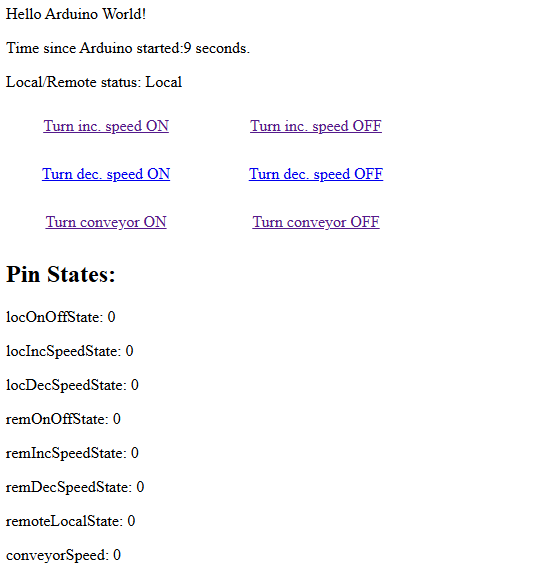
\includegraphics[width=0.8\linewidth]{images/nodeMCUlandingPage.png}
    \caption{Placeholder: Jak vypadá stránka co se objeví pokud zadám IP adresu nodeMCU do prohlížeče}
    \label{fig:NodeMCUlandingPage}
\end{figure}


\source{Vzhledem k tomu, že NodeMCU je open source a mají vlastní dokumentaci tak bych zdroje hledal na jejich webu.}

